\section{Modeling and Solving}

\subsection{Overview}\label{ModelOverview}

In this part, we are going to briefly describe how to model puzzle solving and measure the difficulty of game levels in parallel, using the our model called Model driven by Rule Engine("MRE") to solve Problem I and Problem II.

When solving the Sudoku-like puzzles, such as this "Wonder Island" game, the basic but reasonable thinking pattern is:

\begin{itemize}
  \item To simplify existing rules with the relationship and constraint of rules;
  \item To choose the rule that could contribute solving the most;
  \item To implement this rule and update the "map";
  \item When step 2 could lead to a certain status, to go to step 1 until problem solved;
  \item When step 2 couldn't lead to a certain status, to make each possible assumption as a new status "branch", and go to step 1 trying to solve this branch until puzzle solved or proved self-contradictory.
\end{itemize}

Going through the whole pattern, we found that it could be reflected as a backtracking algorithm, and the step 1 and step 2 mostly infer one's "intelligence" with the main obstacles lying in. Therefore, the key point of the MRE is to measure the complication step 1 and step 2 from the point of human intelligence, and let our algorithm simplify rules then choose best rules consequently. We implement the concepts including conditional entropy, Thinking Energy Cost, and Rule Engine that is described in detail at \ref{Preliminaires}.

Based on our assumptions, we are safe but not certain to say the MRE could carry out every best move and accumulate least complication of those moves, which represents it would apply the smartest strategy. Then with the solving process going on, every move with a difficulty coefficient (to simulate people's trying and backtracking, see\ref{TEC}) will be logged. So when a solution occurred, total TEC could be calculated from the log as a strongly reasonable indicator to measure the difficulty of this game level.

From above, with solving and measuring difficulty based on solving running simultaneously, the MRE is able to accomplish Problem 1 and Problem 2 at once. The whole working precess of the MRE is illustrated in subsection\ref{ModelFramework}.

. In the following sections of this section, we'll discuss about the key points of the MRE: the framework\ref{ModelFramework}, Rule Library simplifying\ref{Pruning}, rule choosing logic\ref{ChoosingRule}, TEC Calculation details\ref{CalcTEC}, and how to transfer the model to solve Problem III\ref{ModelExtend}.

\subsection{The Framework of MRE}\label{ModelFramework}

In this part, we'll demonstrate how the MRE actually works step by step. Firstly, some terms we use in MRE should be described first.

\ref{fig:flow-process diagram}
\begin{figure}[htb]
	\centering
	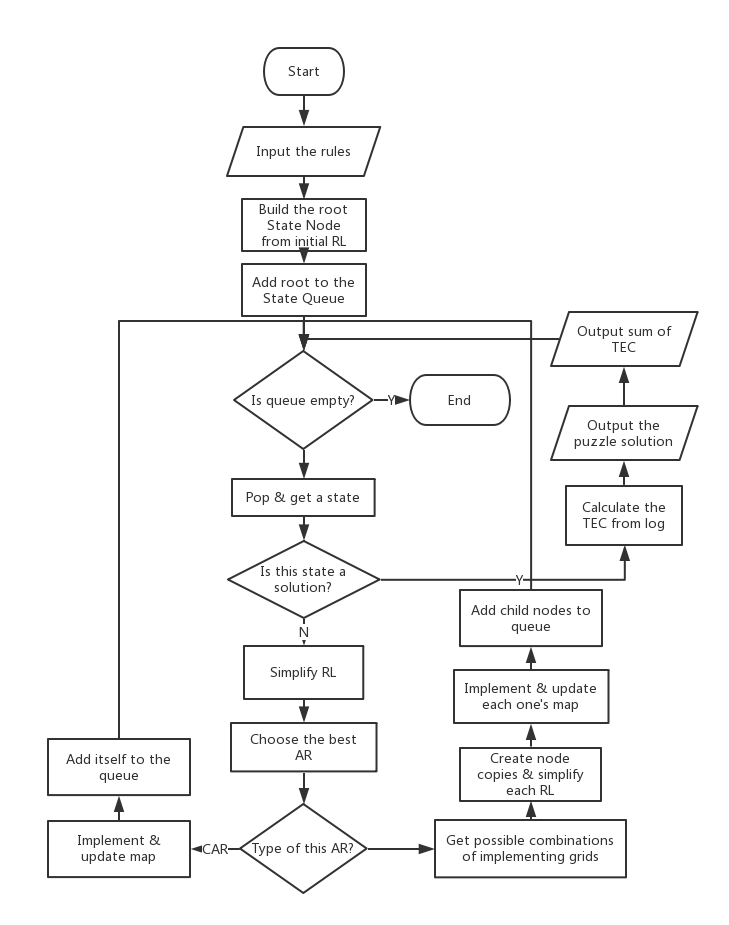
\includegraphics[width=0.7\linewidth]{Figures/MRE Process.png}
	\caption{MRE's Working Process}
	\label{MRE Process}
\end{figure}
